\subsection{Stereovolumenkontrol}
\label{Volumenkontrol}
%
Muligheden for at justere volumen er helt essentiel for det endelige produkt, og derfor skal det implementeres i kredsløbet. Den anvendte stereovolumenkontrol er af typen TDA1524A, hvis datablad er opgivet i \textcite{PDF:VolumeControl}. 

Stereovolumenkontrollen har to inputs og to outputs, da det er beregnet til at justere lyd i stereo, og det er samtidig muligt at regulere balancen mellem disse. Yderligere kan bas og diskant også justeres isoleret, og alle disse parametre justeres med hver deres lineære potentiometer. Stereovolumenkontrollen har en enkelt spændingsforsyning, der må variere mellem 7.5V og 16.5V, \parencite[5]{PDF:VolumeControl}. 
\blankline
På trods af de mange muligheder, som denne type stereovolumenkontrol indeholder, er der i dette projekt afgrænset til udelukkende at anvende det til at justere volumen, altså lydtryksniveauet. Det er derfor nødvendigt at foretage nogle modificeringer på det originale kredsløb, \parencite[3]{PDF:VolumeControl}, særligt for at neutralisere bas og diskant. Da der ikke arbejdes med stereolyd, men mono kortsluttes de to inputs og de to outputs hver for sig, hvilket fremgår af \autoref{fig:Volumen}.

Da hverken bas, diskant eller stereobalance benyttes erstattes deres tilhørende potentiometre med to serielle modstande, som sørger for at der hverken kan skrues op eller ned for de tre funktioner. Det gøres ved at vælg en modstandsværdi som er halvdelen af potentiometerets modstand, da det ville være den ækvivalente modstand til de to serie koblet erstatningsmodstande. Spændingdelingen for hver af de tre funktioner sker mellem $R_3$ og $R_4$, $R_5$ og $R_6$ og mellem $R_7$ og $R_8$, angivet på \autoref{fig:Volumen}. Modstandsværdien for erstatningsmodstandende er på 23.5k$\Omega$.   
%
\begin{figure}[H]
	\centering
	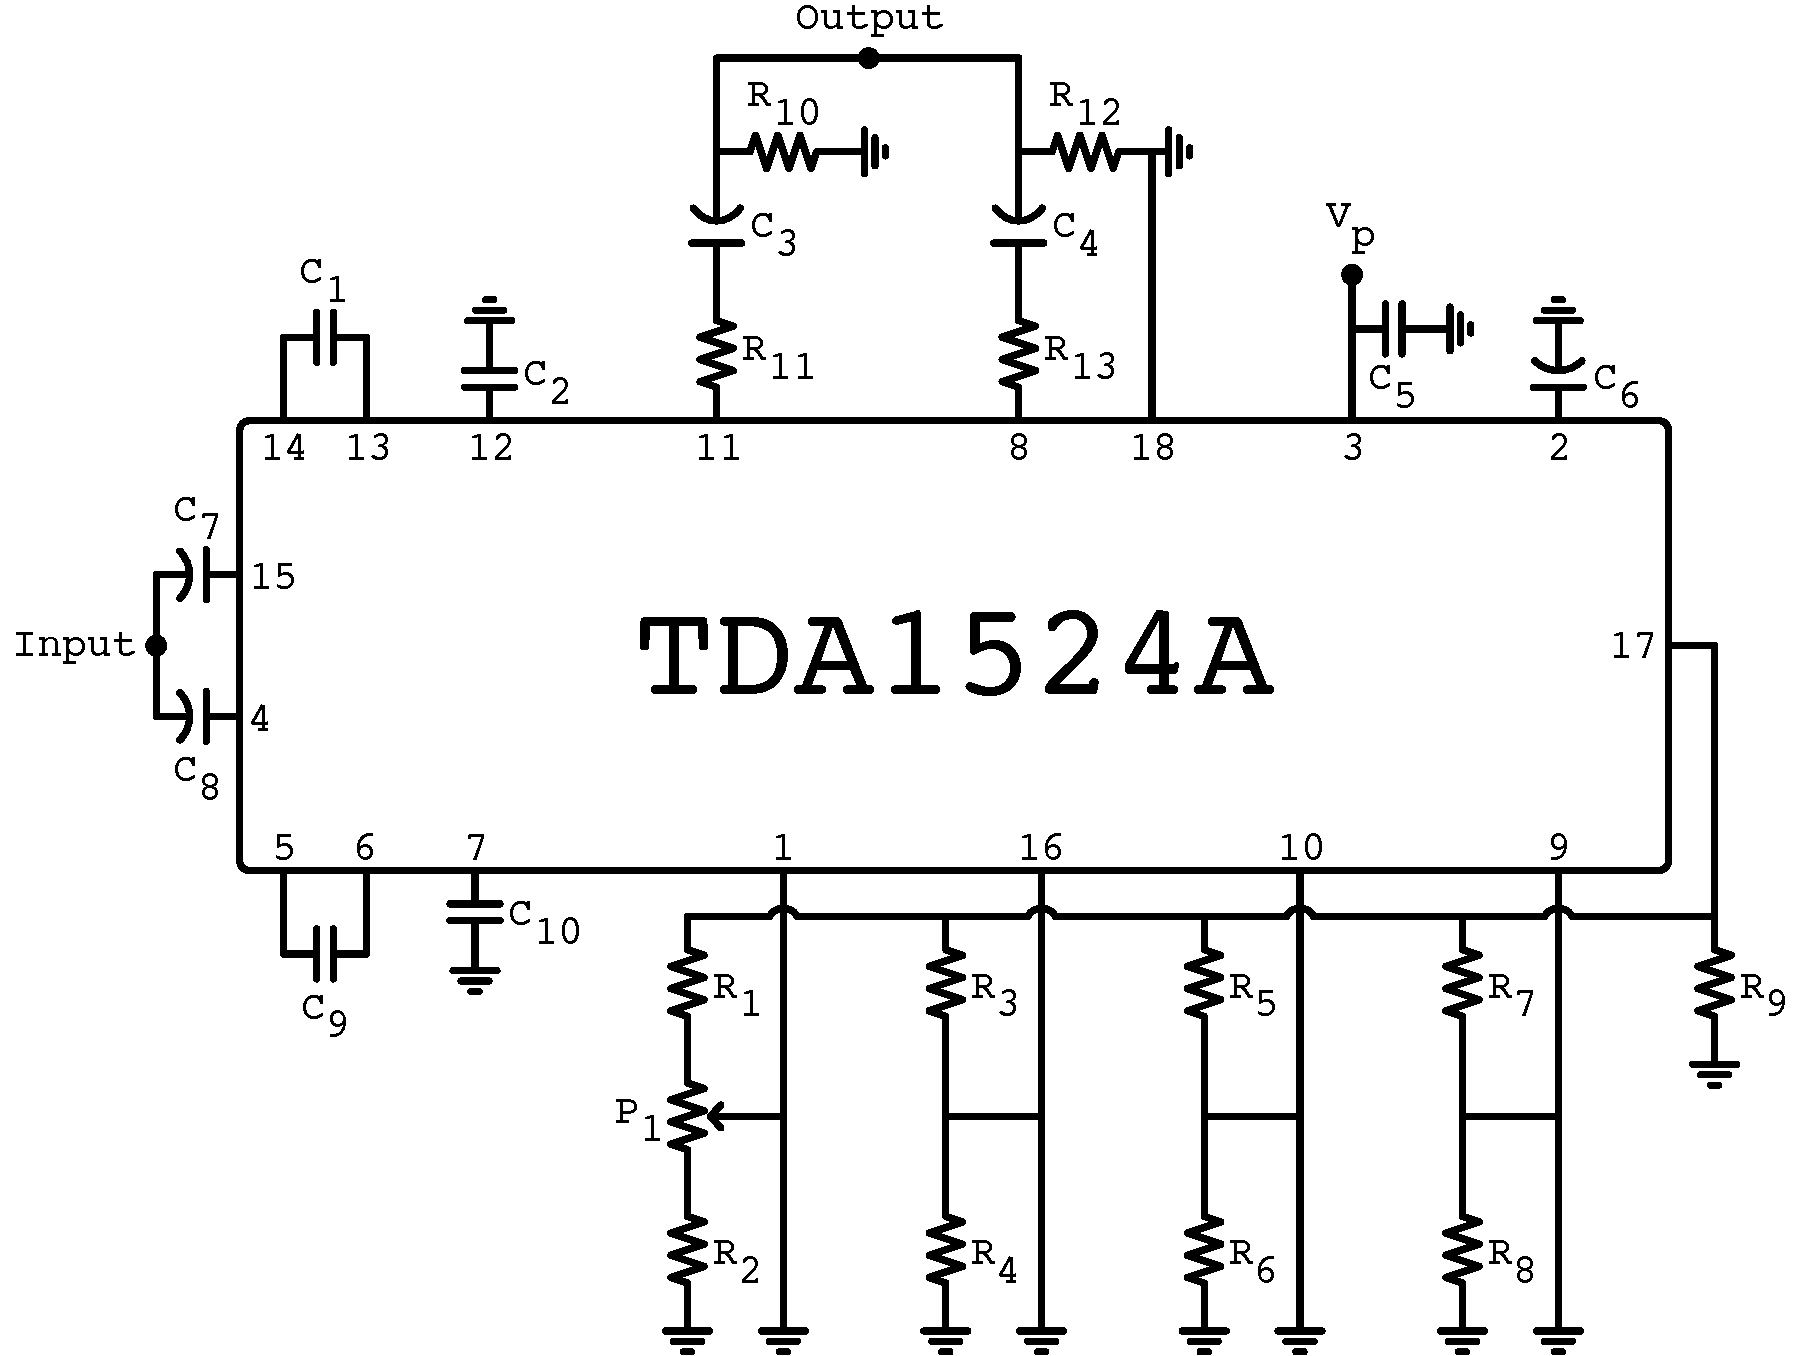
\includegraphics[resolution=300,scale=\circuitSize]{Circuits/Volumen}
	\caption{Kredsløbsdiagram for stereovolumenkontrollen, med de nødvendige justeringer .}
	\label{fig:Volumen}
\end{figure}
\noindent
%
Stereovolumenkontrollen blev først bygget på et fumlebredt med det formål, at have mulighed for let at ændre og eksperimentere med komponentværdierne, samt foretage målinger. Målingerne blev foretaget ved at sende en 1000Hz tone igennem kredsløbet med en forsyningspænding på +10V. Amplitudeværdier blev herefter aflæst på et oscilloskop ved forskellige spændinger over potentiometeret. Efterfølgende sammenholdes målingerne med databladet for at sikre sig, at stereovolumenkontrollen opfører sig efter hensigten, \parencite[s. 9]{PDF:VolumeControl}. Resultatet af disse målinger fremgår af \autoref{fig:MaalingerPaaBreadboard}.
%
\begin{figure}[H]
	\centering
	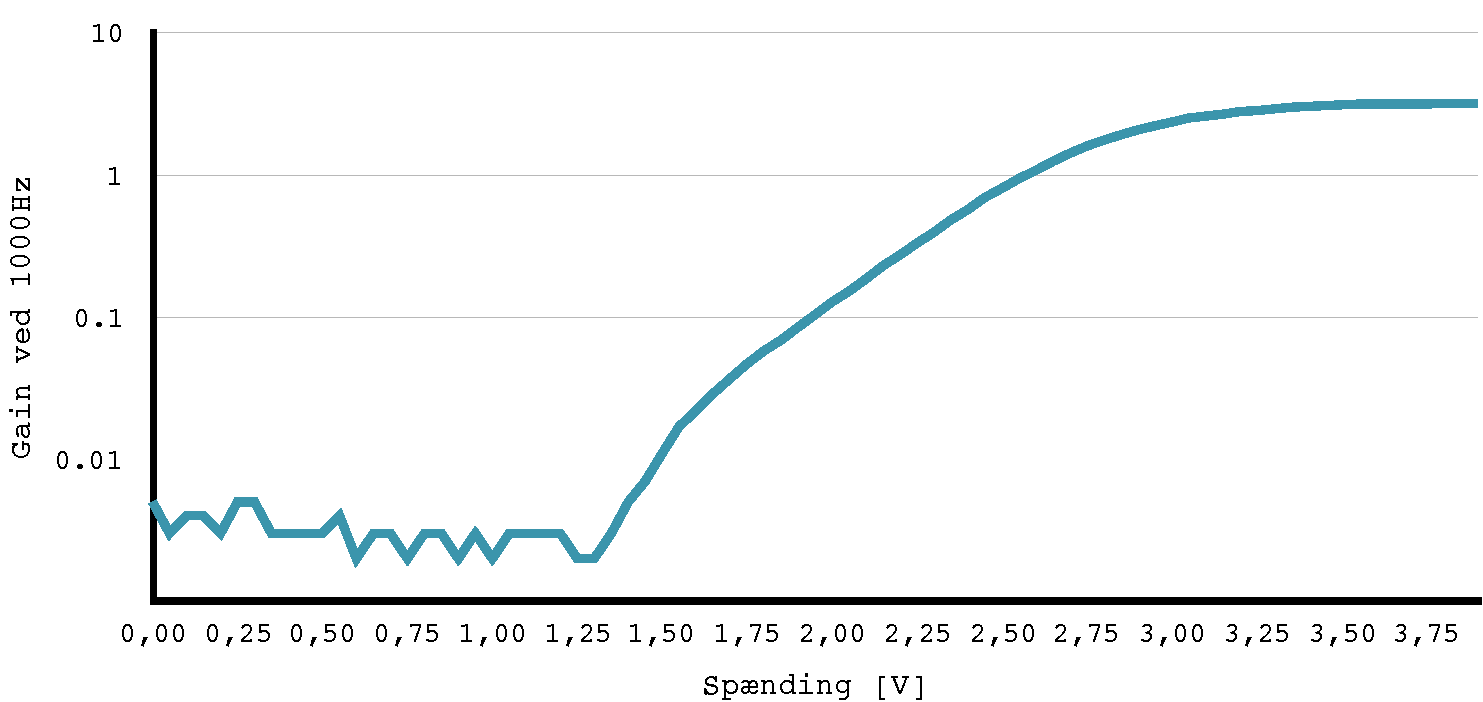
\includegraphics[resolution=300,scale=0.6]{MaalingerAfVolumenkontrol}
	\caption{Målinger foretaget af stereovolumenkontrollen. Hvor x-aksen repræsenterer spændingen over potentiometeret, og y-aksen angiver forstærkningen}
	\label{fig:MaalingerPaaBreadboard}
\end{figure}
\noindent
%
Målet er at der forekommer en lineær udvikling, når der drejes på potentiometeret, hvilket også er tilfældet, dog kun inden for et spektrum mellem ca. 1.25V og 2.85V. Det betyder, at der ikke vil ske en ændring i volumen uden for dette spektrum, hvorfor der ikke forekommer nogle ændringer i starten og slutningen af potentiometerets rotationsakse. Der kompenseres for disse uhensigtsmæssigheder ved at placere passende modstande på hver side af potentiometeret. En modstand på 24.3k$\Omega$ placeres i toppen af potentiometeret og en modstand på 20k$\Omega$ placeres i bunden. Modstandsværdierne blev fundet ved at prøve forskellige værdier til det ønskede resultat blev opnået. Ændringen i opstillingen fremgår ligeledes af \autoref{fig:Volumen}, hvor de pågældende modstande er navngivet $R_1$ og $R_2$.\par
Målingerne efter tilføjelsen fremgår af \autoref{fig:NyeMaalinger}, som gengiver at de to modstande har haft den ønskede effekt; en tilnærmelsesvis lineær udvikling over hele potentiometerets rotationsakse.
%
\begin{figure}[H]
	\centering
	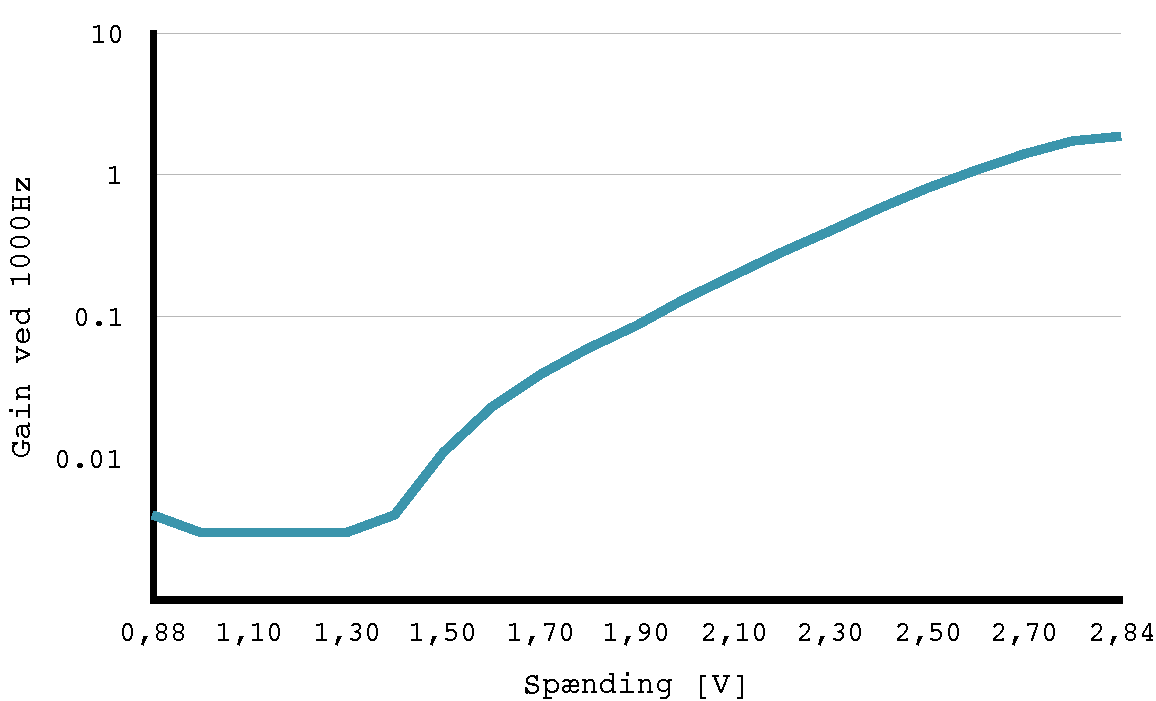
\includegraphics[resolution=300,scale=0.6]{MaalingerAfVolumenkontrolNye}
	\caption{Målinger foretaget af stereovolumenkontrollen efter tilføjelser af modstande på hver side af potentiometeret. Målingerne er foretaget under de samme kriterie, som de første målinger ved at sende en 1000Hz tone gennem med en 10V forsyningsspænding.}
	\label{fig:NyeMaalinger}
\end{figure}
\noindent
%
Som det fremgår af diagrammet for den originale stereovolumenkontrollen, indeholder kredsløbet også en kontakt, der skifter mellem 'contour' og 'linear', hvilket beskriver udviklingen, når der drejes på potentiometeret. Ønsket er en lineær udvikling, når volumen justeres, og derfor kortsluttes kontakten, jævnfør \autoref{fig:Volumen}. Det endelige kredsløb er wrappet, og fremgår af \autoref{fig:VolumenkontrolWrapning}.
%
\begin{figure}[H]
	\centering
	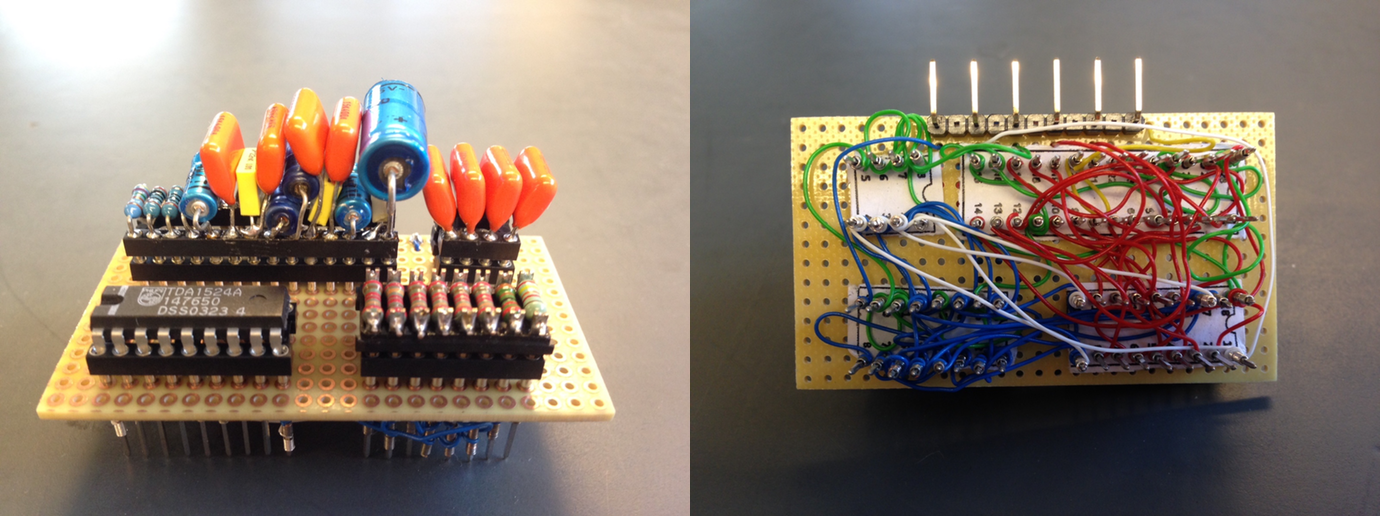
\includegraphics[width=\textwidth]{Volumenkontrol_Wrapning}
	\caption{Opkoblingen af stereovolumenkontrollen ved brug af wrapning. Kredsløbet er fotograferet både fra wrappe siden og komponent siden, hvor komponenterne er loddet i sokler.}
	\label{fig:VolumenkontrolWrapning}
\end{figure}
\noindent